\subsection{Nasi Padang}

Nasi Padang merupakan salah satu bentuk penyajian masakan Minangkabau yang berasal dari Sumatera Barat. Istilah Nasi Padang tidak hanya merujuk pada nasi sebagai makanan utama, tetapi pada penyajian nasi putih bersama beragam masakan pendamping. Masakan tersebut dapat berupa olahan daging, ayam, ikan, sayuran, gulai, dan sambal. Beberapa lauk yang umum dikenal dalam penyajian Nasi Padang antara lain rendang, ayam berbumbu, dan perkedel \cite{yeoh2024nasipadang}. Keragaman tersebut membuat pelanggan dapat memilih jenis dan jumlah lauk sesuai dengan keinginan.

Seporsi Nasi Padang dapat memadukan nasi dengan lauk, kuah gulai, sambal, dan sayuran. Pilihan lauknya dapat berasal dari olahan daging maupun ikan, sedangkan sayur yang disajikan antara lain sayur nangka dan daun singkong \cite{wahyudi2016nasipadang}. Dengan demikian, satu piring Nasi Padang dapat berisi beberapa jenis makanan dengan bentuk, warna, dan tekstur visual yang berbeda.

Pada pelayanan makan di tempat atau \textit{dine-in}, terdapat dua metode penyajian yang dikenal sebagai \textit{hidang} dan \textit{pesan}. Pada metode \textit{hidang}, sejumlah piring kecil yang berisi lauk berbeda dibawa oleh pelayan dan diletakkan di meja pelanggan. Pelanggan kemudian membayar lauk yang dikonsumsi. Sementara itu, pada metode \textit{pesan}, pelanggan memilih lauk dari makanan yang ditampilkan pada etalase, kemudian nasi dan lauk yang dipilih disajikan kepada pelanggan \cite{yeoh2024nasipadang}.

\begin{figure}[H]
    \centering
    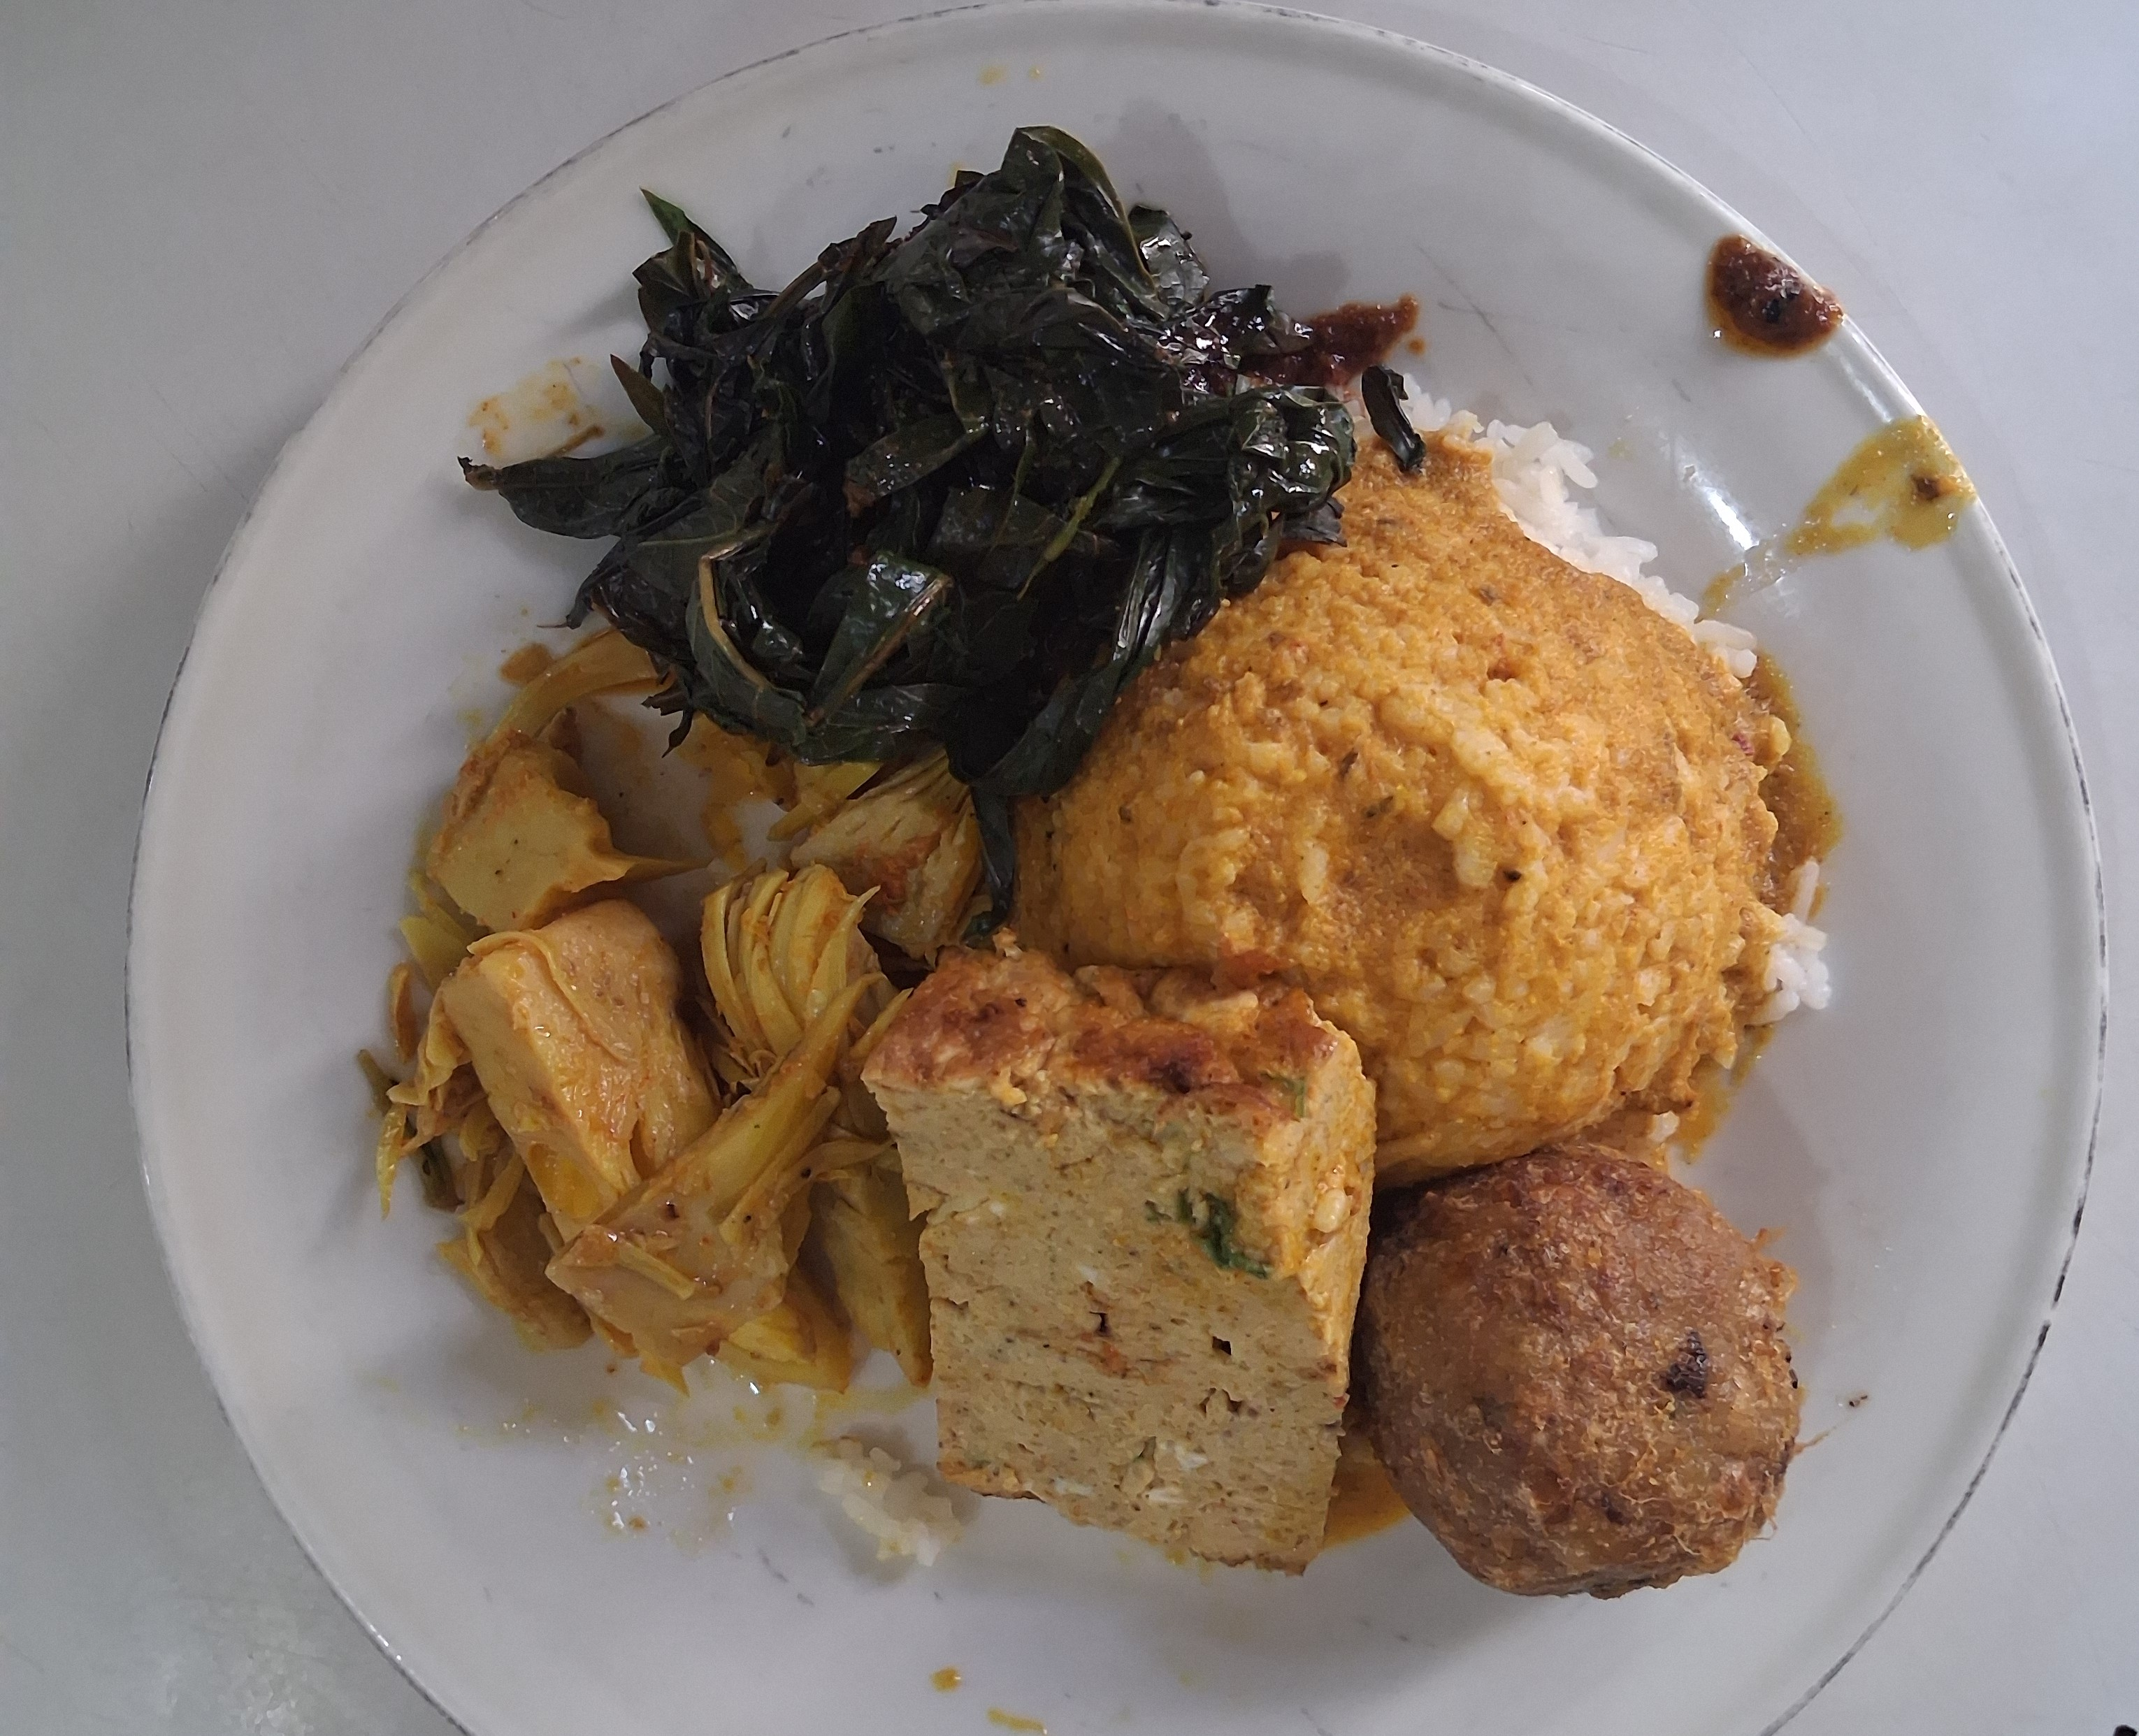
\includegraphics[width=0.5\textwidth]{figures/nasi_padang_dine_in.jpg}
    \caption{Contoh penyajian Nasi Padang untuk pelanggan \textit{dine-in}}
    \label{fig:nasi-padang-dine-in}
		{\footnotesize Sumber: Dokumentasi Pribadi}
\end{figure}

Selain disajikan untuk makan di tempat, Nasi Padang juga dapat disiapkan untuk dibawa pulang atau \textit{take-away}. Pada bentuk penyajian ini, nasi, lauk, sayur, sambal, dan kuah yang dipilih ditempatkan dalam satu bungkus. Penggunaan daun pisang sebagai bagian dari pembungkus juga menjadi salah satu bentuk penyajian Nasi Padang untuk dibawa pulang. Pada sejumlah rumah makan, porsi nasi dalam penyajian bungkus dapat lebih banyak dibandingkan dengan penyajian makan di tempat. Salah satu alasan yang dikemukakan adalah bahwa nasi bungkus pada awalnya dapat dikonsumsi bersama oleh lebih dari satu orang \cite{wahyudi2016nasipadang}.

\begin{figure}[H]
    \centering
    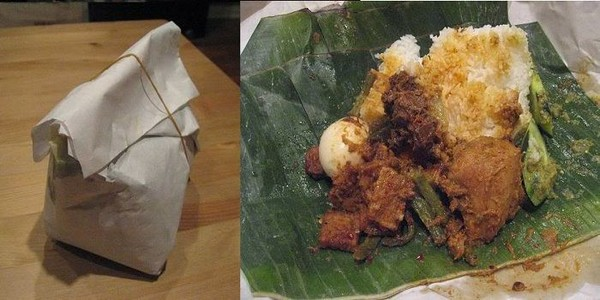
\includegraphics[width=0.55\textwidth]{figures/nasi_padang_take_away.jpeg}
    \caption{Contoh penyajian Nasi Padang untuk \textit{take-away}}
    \label{fig:nasi-padang-take-away}
		{\footnotesize Sumber:
    \href{https://food.detik.com/info-kuliner/d-4876612/ini-arti-kode-yang-tertulis-pada-bungkus-nasi-padang}
    {Fitria, DetikFood (2020)}, diakses 29 Agustus 2026}
\end{figure}

Perbedaan cara penyajian tersebut menghasilkan kondisi visual yang berbeda. Pada penyajian \textit{dine-in}, nasi dan lauk berada dalam kondisi terbuka pada piring sehingga dapat diamati secara langsung dari arah atas. Sebaliknya, pada penyajian \textit{take-away}, seluruh makanan telah digabungkan dan ditempatkan di dalam bungkus. Oleh karena itu, sistem yang dirancang dalam penelitian ini difokuskan pada penyajian \textit{dine-in}. Pembahasan mengenai penyajian \textit{take-away} digunakan untuk memberikan konteks mengenai perbedaan bentuk penyajian Nasi Padang, tetapi tidak termasuk dalam ruang lingkup pengenalan lauk oleh sistem.
